\documentclass[10pt]{article}

\def\HandoutNumber{6}
\def\TheDate{February 5, 2016}
\def\Name{Blake Riley}

\usepackage{amsmath,amsfonts,amsthm,amssymb}
\usepackage{setspace}
\usepackage{graphicx,float,wrapfig}
%\usepackage{parskip}
\usepackage{enumerate}
\usepackage{url}

\usepackage{fourier}
\usepackage[T1]{fontenc}
\usepackage[protrusion=true,expansion=true]{microtype}

% In case you need to adjust margins:
\topmargin=-0.45in      %
\evensidemargin=0in     %
\oddsidemargin=0in      %
\textwidth=6.5in        %
\textheight=9.0in       %
\headsep=0.25in         %
\parindent=0in

\usepackage[nodayofweek]{datetime} \usdate
% Pdf metadata
\pdfinfo{  /Author (\Name)
           /Title (Economics 533 Handout \HandoutNumber)
           /Keywords ()
           /ModDate (D:\pdfdate)}

\newtheoremstyle{basic}% name
   {5pt}% Space above
   {5pt}% Space below
   {\itshape \leftskip=1em}% Body font
   {-1em}% Indent amount
   {\bfseries}% Theorem head font
   {:}% Punctuation after theorem head
   { }% Space after theorem head
   {}% Theorem head spec (can be left empty, meaning `normal')
\theoremstyle{basic}
\newtheorem{exercise}{Exercise}[]
\newtheorem{definition}{Definition}[section]
\newtheorem{theorem}{Theorem}[section]
\newtheorem{lemma}[theorem]{Lemma}

\usepackage{tikz} % For drawing diagrams
\usetikzlibrary{calc}
\tikzset{
% Two node styles for game trees: solid and hollow
solid node/.style={circle,draw,inner sep=1.5,fill=black},
hollow node/.style={circle,draw,inner sep=1.5}
}

%%%%%%%%%%%%%%%%%%%%%%%%%%%%%%%%%%%%%%%%%%%%%%%%%%%%%%%%%%%%

% Custom commands

\newcommand{\R}{\mathbb{R}}
\newcommand{\N}{\mathbb{N}}
\newcommand{\E}{\operatorname{E}}
\renewcommand{\P}{\operatorname{Pr}}
\newcommand{\Var}{\operatorname{Var}}
\newcommand{\Cov}{\operatorname{Cov}}
\newcommand{\cond}{\,|\,}
\newcommand{\bigcond}{\;\big|\;}
\newcommand{\argmax}{\mathop{\operatorname{arg\,max}}}
\newcommand{\noti}{{{\scriptscriptstyle-}\!i}}
\newcommand{\notj}{{{\scriptscriptstyle-}\!j}}
\newcommand{\notij}{{{\scriptscriptstyle-}\!\{i,j\}}}
\newcommand{\I}{\mathbb{I}}
\newcommand{\tto}{\twoheadrightarrow}


%%%%%%%%%%%%%%%%%%%%%%%%%%%%%%%%%%%%%%%%%%%%%%%%%%%%%%%%%%%%%
%%%%%%%%%% The main document content
%%%%%%%%%%%%%%%%%%%%%%%%%%%%%%%%%%%%%%%%%%%%%%%%%%%%%%%%%%%%%

\begin{document}
\begin{spacing}{1.0}

\noindent
\textbf{Handout \HandoutNumber Answers} \\
Econ 533 \\
\TheDate \\
TA: \Name \\

First, to clarify, redistribution mechanism payments\footnote{Conitzer and
  Guo (2008)
  (\url{http://www.cs.duke.edu/~conitzer/undominatedAAMAS08.pdf}) seems to
  be the best reference.} are determined by
  \begin{enumerate}
  \item Calculating the pivotal payments $t_i^p(\theta)$ for each agent.
  \item Calculating the minimal total pivotal payments for some report of
    $i$
    \begin{align*}
      T_i(\theta_\noti) = \min_{\theta_i} \sum_{j=1}^n t_j^p(\theta_i, \theta_\noti)
    \end{align*}
  \item Assigning transfers
    \begin{align*}
      t_i^r(\theta) = t_i^p(\theta) - \frac{1}{n} T_i(\theta_\noti)
    \end{align*}
    where $T_i(\theta_\noti)/n$ is the agent's rebate.
  \end{enumerate}
  Alternatively, we can let $T_i$ be the VCG revenue if the agent did not
  participate at all, which is equivalent in many auction settings.

\vspace{1em}
\noindent
  Describe the VCG family, pivotal mechanism, and redistribution mechanism
outcomes for the following applications:
  \begin{enumerate}
  \item \textit{Living arrangements: Three grad students, Abel, Baker, and
      Charlie, are renting a three-bedroom apartment together. The rent is
      \$600 and they've committed to paying equal shares. Now they have to
      decide who gets the big room, the small room with a view, and the
      small dark room. Abel values the three at an additional \$200,
      \$100, and \$0 respectively, while Baker's valuations are \$100,
      \$60, and \$0 and Charlie's valuations are \$25, \$0, and \$50. Now
      suppose Charlie's valuations are \$150, \$25, and \$0.}

  In the first case, the efficient allocation is $(b, v, d)$, with the big
  room going to A, the room with a view going to B, and the dark room
  going to C. The family of VCG payments for this type profile is

  \begin{tabular}{ll}
    $t_A$ & $60 + 50 + h_A$ \\
    $t_B$ & $200 + 50 + h_B$ \\
    $t_c$ & $200 + 60 + h_C$
  \end{tabular}

  where the individualized taxes are single-valued since we are only
  considering a single type profile. The pivotal mechanism payments are

  \begin{tabular}{lll}
    $t_A^p$ & $60 + 50  - (100 + 50)$ & $= -40$ \\
    $t_B^p$ & $200 + 50 - (200 + 50)$ &= 0 \\
    $t_C^p$ & $200 + 60 - (200 + 60)$ &= 0
  \end{tabular}

  since A is pivotal in preventing B from having the big room, causing an
  externality of \$40.

  For the redistribution mechanism, total VCG mechanism payments are going
  to be minimized when an agent reports all valuations as zero. If A
  reports all as zero, there is no incentive conflict, so payments are
  zero and A gets no rebate. If B reports all zeros, again no VCG payments
  and no rebate for B. If C reports all zeros, the total payments will
  be \$40, so C gets a rebate of \$40/3:

  \begin{tabular}{lll}
    $t_A^r$ & $= -40 - 0$ & $=-40$ \\
    $t_B^r$ & $= 0 - 0$ & $=0$ \\
    $t_C^r$ & $= 0 + 40/3$ & $\simeq 13$
  \end{tabular}

  In the second case, the efficient allocation is still $(b, v, d)$. The
  family of VCG payment for this profile is

  \begin{tabular}{ll}
    $t_A$ & $60 + 0 + h_A$ \\
    $t_B$ & $200 + 0 + h_B$ \\
    $t_C$ & $200 + 60 + h_C$
  \end{tabular}

  The pivotal mechanism payments are

  \begin{tabular}{lll}
    $t_A^p$ & $60 - (150 + 60)$ & $= -150$ \\
    $t_B^p$ & $250 - (100 + 150)$ & $= -50$ \\
    $t_C^p$ & $260 - (200 + 60)$ &= 0
  \end{tabular}

  since A is pivotal in preventing C from having the big room and B is
  pivotal in preventing C from getting the big room and A getting the
  view.

  For the redistribution mechanism, if A had all zero valuations, the
  allocation would be $(d, v, b)$ and C would be pivotal, yielding \$40 in
  revenue. If B had all zero valuations, the allocation would be $(v, d,
  b)$ and C would again be pivotal, yielding \$100 in revenue this time
  since the externality against A is larger than against B. If C reported
  all zeros, the total revenue would be \$40. Then the redistribution
  mechanism payments are

  \begin{tabular}{lll}
    $t_A^r$ & $= -150 + 40/3$ & $\simeq -137$ \\
    $t_B^r$ & $= -50 + 100/3$ & $\simeq -17$ \\
    $t_C^r$ & $= 0 + 40/3$ & $\simeq 13$
  \end{tabular}

\item \textit{Combinatorial auction: Later, during finals season when no
    one has time to go shopping, the roommates discover the only things
    left in their refrigerator are a slice of ham, a carrot, and a can of
    PBR. Abel values the slice of ham and the PBR jointly at \$6, but
    would rather get nothing than any single item. Baker is a vegetarian
    and values the carrot and the PBR at \$4, the carrot at \$1, and the
    PBR at \$2. Charlie is only after the PBR, which he values at \$4.}

  The efficient allocation is the ham and PBR to A and the carrot to
  B. The family of VCG payments is

  \begin{tabular}{ll}
    $t_A$ & $1 + 0 + h_A$ \\
    $t_B$ & $6 + 0 + h_B$ \\
    $t_C$ & $6 + 1 + h_C$
  \end{tabular}

  The pivotal payments are

  \begin{tabular}{lll}
    $t_A^p$ & $1 - (1 + 4)$ & $= -4$ \\
    $t_B^p$ & $6 - (6 + 0)$ & $= 0$ \\
    $t_C^p$ & $7 - (6 + 1)$ &= 0
  \end{tabular}

  If A reported zero valuations for all possible allocations, the VCG
  allocation would be the PBR to C and the carrot to B. The total revenue
  would be \$3 since C is pivotal in blocking the PBR and carrot to
  B. If B reports zero valuations, VCG revenue is \$4. If C reports zeros,
  the VCG revenue is \$3. Then the redistribution mechanism payments are

  \begin{tabular}{lll}
    $t_A^r$ & $= -4 + 3/3$ & $= -3$ \\
    $t_B^r$ & $= 0 + 4/3$ & $= 4/3$ \\
    $t_C^r$ & $= 0 + 3/3$ & $= 1$
  \end{tabular}

\item \textit{Buying a path in a network: Consider a series of roads
    between towns modeled as a weighted directed graph
    $G=(V,\mathcal{E})$, where each road $e\in \mathcal{E}$ is owned by a
    local Baron and has a cost $c_e \geq 0$ if the road is used by the
    King's Army. Suppose we want to procure a path for soldiers between
    two towns $A,F \in V$. How should the King's economists compensate the
    Barons for routing the army through their fiefdoms?}
    \begin{center}
      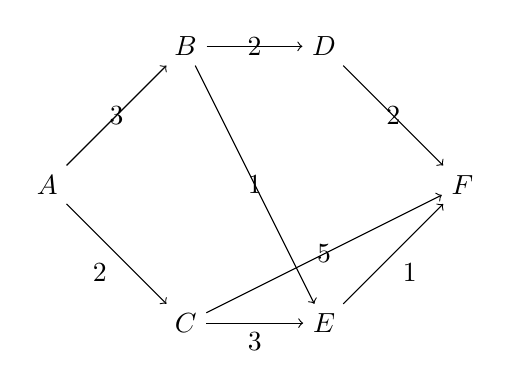
\begin{tikzpicture}[node distance=5em]
        \node (a) {$A$};
        \node (b) [right of=a, above of=a] {$B$};
        \node (c) [right of=a, below of=a] {$C$};
        \node (d) [right of=b] {$D$};
        \node (e) [right of=c] {$E$};
        \node (f) [right of=d, below of=d] {$F$};
        \draw[->] (a) to node {3} (b);
        \draw[->] (a) to node [below left]{2} (c);
        \draw[->] (b) to node {2} (d);
        \draw[->] (b) to node {1} (e);
        \draw[->] (c) to node [below]{3} (e);
        \draw[->] (c) to node {5} (f);
        \draw[->] (d) to node {2} (f);
        \draw[->] (e) to node [below right]{1} (f);
      \end{tikzpicture}
    \end{center}

    The minimum cost path is $A\to B \to E \to F$. Since these are costs,
    not valuations, the VCG family of payments is

    \begin{tabular}{ll}
    $t_{AB}$ & $-1 -1 + h_A$ \\
    $t_{AC}$ & $-3-1-1 + h_B$ \\
    $t_{BD}$ & $-3-1-1 + h_A$ \\
    $t_{BE}$ & $-3-1 + h_A$ \\
    $t_{CE}$ & $-3-1-1 + h_A$ \\
    $t_{CF}$ & $-3-1-1 + h_A$ \\
    $t_{DF}$ & $-3-1-1 + h_A$ \\
    $t_{EF}$ & $-3-1 + h_A$
    \end{tabular}

    The pivotal payments are

    \begin{tabular}{lll}
    $t_{AB}^p$ & $-2 - (-2-3-1)$ &= 4\\
    $t_{AC}^p$ & $-5 - (-3-1-1)$ &= 0\\
    $t_{BD}^p$ & $-5 - (-3-1-1)$ &= 0\\
    $t_{BE}^p$ & $-4 - (-2-3-1)$ &= 2\\
    $t_{CE}^p$ & $-5 - (-3-1-1)$ &= 0\\
    $t_{CF}^p$ & $-5 - (-3-1-1)$ &= 0\\
    $t_{DF}^p$ & $-5 - (-3-1-1)$ &= 0\\
    $t_{EF}^p$ & $-4 - (-2-5) $  &= 3
  \end{tabular}

  The redistribution mechanism in this setting is a bit tricky, both in
  what it represents and how to calculate the payments. I think the
  redistribution mechanism here minimizes the King's total payment while
  ensuring the King doesn't make money off the mechanism. VCG payments are
  minimized when an agent's cost makes the minimum cost path including
  their edge equal in weight to the minimum cost path excluding their
  edge. For instance, revenue is minimized when the cost of AB is 4, which
  makes ABEF equal ACEF at a cost of 6 total. Then, the total VCG revenue
  would be 7, so AB can get a rebate (in this case an extra charge) of
  7/8. Doing this for all agents yields

  \begin{tabular}{ll}
    $t_{AB}^r$ &= $4 - 7/8$ \\
    $t_{AC}^r$ &= $0 - 7/8$ \\
    $t_{BD}^r$ &= $0 - 2/8$ \\
    $t_{BE}^r$ &= $1 - 7/8$ \\
    $t_{CE}^r$ &= $0 - 7/8$ \\
    $t_{CF}^r$ &= $0 - 5/8$ \\
    $t_{DF}^r$ &= $0 - 6/8$ \\
    $t_{EF}^r$ &= $3 - 7/8$
  \end{tabular}

  which has a total payment to the Barons of 2 rather than 8.

\item \textit{Multi-unit auction: $k$ units of an identical good are up
    for sale and each buyer has a valuation $v_i$ for a single item.}

  The efficient allocation is the $k$-th highest bidders receiving an item
  (with some tie-breaking rules). Then, the VCG family is
  \begin{align*}
    t_i(v) = \sum_{j \ne i} v_j \mathbb{I}(v_j \ge v_{(n-k+1)}) + h_i(v_{-i})
  \end{align*}

  The VCG payments are
  \begin{align*}
    t_i(v) &=
      \begin{cases}
        \sum_{j \ne i} v_j \mathbb{I}(v_j \ge v_{(n-k+1)}) - \sum_{j \ne i}
        v_j \mathbb{I}(v_j \ge v_{(n-k)}) & \mbox{if $i$ gets an item} \\
        \sum_{j \ne i} v_j \mathbb{I}(v_j \ge v_{(n-k+1)}) - \sum_{j \ne i}
        v_j \mathbb{I}(v_j \ge v_{(n-k+1)}) & \mbox{if $i$ doesn't get
          an item}
      \end{cases} \\
      & =
      \begin{cases}
        -v_{(n-k)} & \mbox{if $i$ gets an item} \\
        0 & \mbox{if $i$ doesn't get an item}
      \end{cases}
  \end{align*}

  If someone with valuation $v_i \ge v_{(n-k)}$ had reported zero, the
  total revenue becomes $k v_{(n-k-1)}$, and otherwise total revenue is
  unchanged at $k v_{(n-k)}$, so redistribution mechanism payments are

  \begin{align*}
    t_i(v) &=
      \begin{cases}
        - v_{(n-k)} + \frac{k}{n} v_{(n-k-1)} & \mbox{if $i$ gets an item} \\
        \frac{k}{n} v_{(n-k-1)} & \mbox{if $i$ is the highest bidder not
          getting an item} \\
        \frac{k}{n} v_{(n-k)} & \mbox{if $i$ doesn't get an item}
      \end{cases}
  \end{align*}

\end{enumerate}

%%%%%%%%%%%%%%%
\end{spacing}
\end{document}
%%%%% FIN %%%%%
%%%%%%%%%%%%%%%